
%(BEGIN_QUESTION)
% Copyright 2012, Tony R. Kuphaldt, released under the Creative Commons Attribution License (v 1.0)
% This means you may do almost anything with this work of mine, so long as you give me proper credit

This simplified PFD shows the {\it fluid catalytic cracking} or {\it FCC} process, used extensively in American oil refineries.  FCC processes employ finely-powdered catalyst to accelerate chemical reactions where heavy liquid hydrocarbon molecules are split (``cracked'') into lighter molecules, producing petroleum liquids with greater market value.  This is not unlike the chemical process of {\it biomass gasification}, where solid fuel materials are broken down by intense heat into simpler, flammable gases with more flexible application as fuels:

$$\includegraphics[width=15.5cm]{i01120x01.eps}$$

The cracking reactions begin in the riser and continue in the reactor, with the catalyst powder carried along by the steam and hydrocarbon fluids.  These reactions leave much of the catalyst powder covered with coke (solid carbon deposits) which limits its effectiveness as a catalyst.  This ``spent'' catalyst falls by gravity into the regenerator, where it encounters a blast of air entering the bottom of the vessel, converting the carbon deposits into CO and CO$_{2}$ gases and ``fluidizing'' the catalyst powder once again so it flows freely back to the riser.  The hot gases leaving the regenerator pass through a heat exchanger to boil water into useful steam, then pass to a burner where more air is introduced to convert the CO gas into CO$_{2}$ gas and generate more steam with the heat.  Vapors leaving the top of the reactor vessel are distilled into their constituent compounds in the fractionator vessel, with the heaviest of them recycled back to the reactor for re-processing.

\vskip 10pt

Identify appropriate instrumentation technologies for each of the following measurement points:

\begin{itemize}
\item{} Hydrocarbon feed flow
\item{} Stripping steam flow measurement
\item{} Regenerator air flow
\item{} Regenerated catalyst flow
\item{} Recycle slurry flow
\item{} CO concentration to steam generator
\item{} Oxygen concentration inside regenerator
\item{} NO$_{x}$ emissions from CO boiler
\end{itemize}

\underbar{file i01120}
%(END_QUESTION)





%(BEGIN_ANSWER)

The following suggestions are not necessarily the {\it only} possible choices for each application:

\begin{itemize}
\item{} Hydrocarbon feed flow: {\it orifice plate}
\vskip 10pt
\item{} Stripping steam flow measurement: {\it vortex flowmeter}
\vskip 10pt
\item{} Regenerator air flow: {\it pitot tube}
\vskip 10pt
\item{} Regenerated catalyst flow: {\it Doppler ultrasonic}
\vskip 10pt
\item{} Recycle slurry flow: {\it Segmental wedge}
\vskip 10pt
\item{} CO concentration to steam generator: {\it NDIR (with filter cells!)}
\vskip 10pt
\item{} Oxygen concentration inside regenerator: {\it paramagnetic}
\vskip 10pt
\item{} NO$_{x}$ emissions from CO boiler: {\it chemiluminescence}
\end{itemize}


%(END_ANSWER)





%(BEGIN_NOTES)


%INDEX% Process: fluid catalytic cracker (oil refinery)

%(END_NOTES)


